\documentclass{article}

% Language setting
% Replace `english' with e.g. `spanish' to change the document language
\usepackage[english]{babel}

% Set page size and margins
% Replace `letterpaper' with `a4paper' for UK/EU standard size
\usepackage[letterpaper,top=2cm,bottom=2cm,left=3cm,right=3cm,marginparwidth=1.75cm]{geometry}

% Useful packages
\usepackage{amsmath}
\usepackage{graphicx}
\usepackage{svg}
\usepackage[colorlinks=true, allcolors=blue]{hyperref}
\usepackage{braket} % Dirac notation packet
\usepackage{comment} % to comment large sections
\usepackage{mhchem} % left superscripts
\usepackage{subcaption} % use subfigures see: https://tex.stackexchange.com/questions/200994/environment-subfigure-undefined-on-journal-submission
\captionsetup{compatibility=false} % use subfigures

% Define inverse trigonometric functions
\DeclareMathOperator{\sech}{sech}
\DeclareMathOperator{\csch}{csch}

%%%%%%%%%%%%%%%%%%%%%%%%%%%%%%%%%%%%%%%%%%%%%%%%%%%
% python code
\usepackage{listings}
\usepackage{color}
\usepackage{xcolor}

\definecolor{codegreen}{rgb}{0,0.6,0}
\definecolor{codegray}{rgb}{0.5,0.5,0.5}
\definecolor{codepurple}{rgb}{0.58,0,0.82}
\definecolor{backcolour}{rgb}{0.95,0.95,0.92}

\lstdefinestyle{mystyle}{
    backgroundcolor=\color{backcolour},
    commentstyle=\color{codegreen},
    keywordstyle=\color{magenta},
    numberstyle=\tiny\color{codegray},
    stringstyle=\color{codepurple},
    basicstyle=\ttfamily\footnotesize,
    breakatwhitespace=false,
    breaklines=true,
    captionpos=b,
    keepspaces=true,
    numbers=left,
    numbersep=5pt,
    showspaces=false,
    showstringspaces=false,
    showtabs=false,
    tabsize=2
}

\lstset{style=mystyle}
%%%%%%%%%%%%%%%%%%%%%%%%%%%%%%%%%%%%%%%%%%%%%%%%%%%

%%%%%%%%%%%%%%%%%%%%%%%%%%%%%%%%%%%%%%%%%%%%%%%%%%%
\usepackage{titlesec} % use paragraphs with numbers
\setcounter{secnumdepth}{4}
\titleformat{\paragraph}
{\normalfont\normalsize\bfseries}{\theparagraph}{1em}{}
\titlespacing*{\paragraph}
{0pt}{3.25ex plus 1ex minus .2ex}{1.5ex plus .2ex}
%%%%%%%%%%%%%%%%%%%%%%%%%%%%%%%%%%%%%%%%%%%%%%%%%%%

\title{Title}
\author{Edgar Zuniga}

\begin{document}
\maketitle
\tableofcontents

\begin{abstract}
Your abstract.
\end{abstract}

\section{Light Gravimeter}
\subsection{Gravitational redshift}
The gravitational redshift (GR) is the frequency shift of an electromagnetic wave due to a change in the gravitational potential. The frequency(wavelength) of a light ray escaping from a gravitational field will be detected with a lower(higher) frequency(wavelength) at a lower potential \cite{Cheng2004-tw}. This effect is a consequence of the Strong Equivalence Principle (SEP) also known as the Einstein Equivalence Principle\footnote{The EEP states that an inertial reference frame in a (uniform) gravitational field is equivalent for all physical processes to a (suitable) uniformly accelerated reference frame free from gravitational fields \cite{Nobili-2013, michael2016}.} (EEP) \cite{Nobili-2013}, and therefore, it can be derived from General Relativity. However, according to the Schiff conjecture\footnote{According to the Schiff conjecture, every relativistic theory that satisfies the WEP necessarily satisfies the EEP.} \cite{coley-1982}, by considering that the Weak Equivalence Principle\footnote{The WEP states that the inertial and gravitational masses are equivalent.} (WEP) applies to clocks and normal matter alike, this effect can be derived solely from Special Relativity (SR) and the WEP \cite{Nobili-2013}.

Consider an electromagnetic wave with wave number $k_{0}$ escaping from a gravitational potential. According to the GR, the wave number will be shifted as the gravitational potential changes according to \cite{Cheng2004-tw}

\begin{equation}
    k = k_{0}\bigg(1 - \frac{\Delta V}{c^{2}}\bigg),
\end{equation}
%
where $\Delta V$ is the change in the gravitational potential, and $c$ is the speed of light. Notice that we have decided to write the GR in terms of the wave number because this form will be helpful in the next sections but we could have written it in terms of the frequency or wavelength as well.


\subsection{Review of the interference term}
In this section, we will give a brief review of optical interference \footnote{A wider reference to the phenomena of interference can be found in many textbooks, here, we follow Ref. \cite{Hecht2016-lx}.}. This discussion will be relevant later when we introduce the light gravimeter. Consider two linearly polarized plane waves of the form

\begin{equation}
\label{plane_waves}
    \begin{aligned}
    \Vec{E_{1}}(\Vec{r}, t) &= \Vec{E_{01}} \cos (\Vec{k_{1}} \cdot \Vec{r} - \omega t + \varphi_{1}), \\
    \Vec{E_{2}}(\Vec{r}, t) &= \Vec{E_{02}} \cos (\Vec{k_{2}} \cdot \Vec{r} - \omega t + \varphi_{2}),
    \end{aligned}
\end{equation}
%
where $\omega$ is the angular frequency, $\Vec{r}$ is the position vector, $t$ is the time, $\Vec{k_{i}}$ is the wave vector, $\varphi_{i}$ is a phase offset, and $\Vec{E_{0i}}$ is the electric field amplitude of the waves $i=1,2$. When these waves interfere at a point $\Vec{r}$ at time $t$, the detector measures the irradiance of the superposition $\Vec{E} = \Vec{E_{1}} + \Vec{E_{2}}$ given by the time-averaged value of the squared magnetic field amplitude

\begin{equation}
    I \sim \braket{\Vec{E}^{2}}_{T},
\end{equation}
%
where the time averaged value of a function $f(t)$ is given by

\begin{equation}
\label{averaged_function}
    \braket{f(t)}_{T} = \frac{1}{T} \int_{t-T/2}^{t+T/2} f(t) \,dt.
\end{equation}
%
Thus, the irradiance can be written as

\begin{equation}
    I = I_{1} + I_{2} + I_{12},
\end{equation}
%
where

\begin{equation}
    \begin{aligned}
        I_{1} &= \braket{\Vec{E_{1}}^{2}}_{T},\\
        I_{2} &= \braket{\Vec{E_{2}}^{2}}_{T},\\
        I_{12} &= 2 \braket{\Vec{E_{1}} \cdot \Vec{E_{2}}^{2}}_{T}.
    \end{aligned}
\end{equation}
%
The term $I_{12}$ is known as the interference term and is responsible for the interference pattern. We can perform the integral in Eq. \ref{averaged_function} by considering that the period of integration of the sensor $T$ is much larger than the period of oscillation $\tau$ of the plane waves, i.e., $T \gg \tau = 2\pi/\omega$ to get

\begin{equation}
    I_{12} = \Vec{E_{01}} \cdot \Vec{E_{02}} \cos \Phi,
\end{equation}
%
where $\Phi$ is the phase difference given by

\begin{equation}
\label{phase_difference_eq}
    \Phi = \Vec{k_{1}} \cdot \Vec{r} - \Vec{k_{2}} \cdot \Vec{r} + \varphi_{1} - \varphi_{2}.
\end{equation}
%
Thus, the phase difference is given by the sum of the difference in path length and the difference in initial phase offset. Notice that when $\Phi = 0,\pm 2\pi,\pm4\pi\ldots$, we have total constructive interference while when $\Phi = \pm\pi,\pm 3\pi,\pm 5\pi\ldots$, we have total destructive interference. This result is general and also holds for spherical waves

\begin{equation}
\label{plane_waves_spherical}
    \begin{aligned}
    \Vec{E_{1}}(\Vec{r_{1}}, t) &= \Vec{E_{01}}(r_{1}) \exp [i (kr_{1} - \omega t + \varphi_{1})], \\
    \Vec{E_{2}}(\Vec{r_{2}}, t) &= \Vec{E_{02}}(r_{2}) \exp [i (kr_{2} - \omega t + \varphi_{2})],
    \end{aligned}
\end{equation}
%
with

\begin{equation}
    \Phi = k(r_{1} - r_{2}) + (\varphi_{1} - \varphi_{2}),
\end{equation}
%
where $r_{1}$ and $r_{2}$ are the radius of the spherical wavefronts overlapping at point P.

Notice that the conditions for the interference term to not depend on $\omega$ are that during the time interval of integration, $\omega$ has to be constant and equal for both waves. Thus, the interference pattern only has a dependence on the difference of path length and the initial phase offset. Later, we will consider that one of the two waves of Eq. \ref{plane_waves} is redshifted during its time travel. In that case, the conditions are still fulfilled if they interfere in a spatial point where $\omega$ is equal for both and the redshift will only cause an increase in the path length traveled by one of the waves causing a phase shift in the fringes.

\subsection{Overview of the light gravimeter}

\begin{figure}
\centering
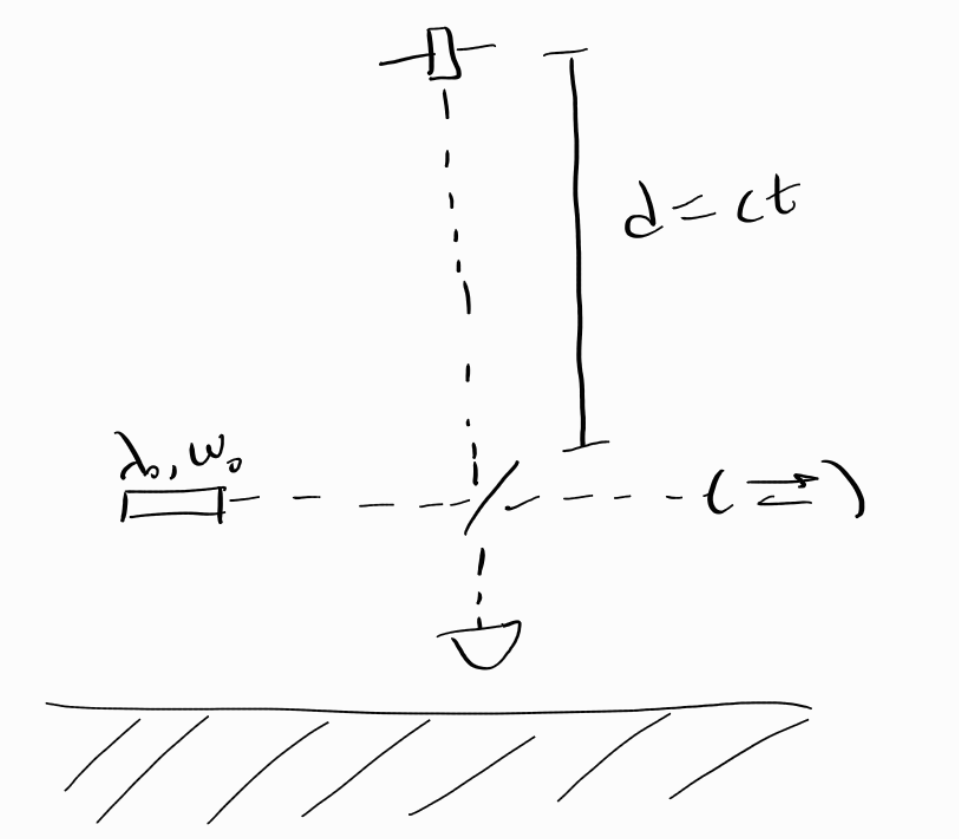
\includegraphics[width=0.6\textwidth]{experimental_setup.png}
\caption{The experimental setup of the light gravimeter consists of a Michelson interferometer with a laser of wavelength $\lambda_{0}$. One arm of the interferometer stays on earth and its optical path length is controlled, for example, through an optical cavity. The other arm of the interferometer acts as a probe of the gravitational field, extending out of the earth's gravitational field and suffering from a GR while escaping from the potential. This beam is retroreflected after it has traveled a distance $d$ from the beam-splitter and returns towards the earth's surface where it interferes with the arm that did not suffer a GR and an interference pattern is measured. Notice that both beams have the same wavelength at the moment when they interfere.}
\label{light_gravimeter_exp_setup_figure}
\end{figure}

In this section, we show how to leverage the GR to measure the local acceleration of gravity ($g$). Our focus will be to introduce the idea of a light gravimeter, thus, we will use unrealistic approximations and leave a more thorough calculation (including corrections) for the next sections. Consider the experimental setup of Fig. \ref{light_gravimeter_exp_setup_figure}. consisting of a Michelson interferometer. A laser of wavelength $\lambda_{0}$, as measured on the earth's surface, is split into two pulses. One arm of the interferometer is kept on the ground and its optical path length can be controlled by using, for example, an optical cavity. The other arm of the interferometer, of length $d$, extends out of the earth's gravitational potential and suffers a GR. Thus, it acts as a probe of the gravitational field as it travels towards outer space. This beam is retroreflected and sent back to the earth's surface where it interferes with the arm that did not suffer a GR. Now, we show that it is possible to extract the value of $g$ corresponding to the location at which the split of the original beam took place.

The phase difference of the interference pattern measured by the detector is given by Eq. \ref{phase_difference_eq}. However, the wavelength of the arm that travels out of the gravitational potential is not constant, furthermore, it depends on the altitude due to the GR. Therefore, we have to take into account all the infinitesimal contributions $\Vec{k} \cdot \Vec{dz}$ to the phase. Thus, the phase difference is more generally given by

\begin{equation}
    \phi = \int k dz,
\end{equation}
%
where we have considered that $\Vec{k} \parallel \Vec{dz}$ and that $\varphi_{1} = \varphi_{2}$. the arms that stays has a phase... but for the other arm .. two contributions given by...

\subsection{Corrections to the gravitational potential}

\subsubsection{Correction due to the shape of the earth}
\subsubsection{Validity of the approximation g$\Delta$z for long distances}
\subsubsection{Contribution of the moon and sun}

\subsection{Phase of the light gravimeter for the earth-moon-sun system}

\subsection{Approximations to the phase of the light gravimeter}

\subsubsection{Case 1}
\subsubsection{Case 2}
\subsubsection{Case 3}
\subsubsection{Case 4}
\subsubsection{Case 5}

\subsubsection{Validity of the approximations}

\subsection{Light vs matter gravimeters}

\subsection{Atmospheric considerations}
The principal source of error in lunar laser ranging is the atmosphere \cite{mingyue2022_DLLR} ...

\subsubsection{Phase shift due to the air refractive index}
\subsubsection{Atmospheric refraction}
\subsubsection{Scattering of light}
\subsubsection{Atmospheric windows}

\subsection{Light beam considerations}
\subsubsection{Coherence length}
\subsubsection{Rayleigh length}


\bibliographystyle{plain}
\bibliography{cites.bib}

\end{document}